%============================================================================
% tento soubor pouzijte jako zaklad
% (c) 2008 Michal Bidlo
% E-mail: bidlom AT fit vutbr cz
%============================================================================
% kodovaní: iso-8859-2 (zmena prikazem iconv, recode nebo cstocs)
%----------------------------------------------------------------------------
% zpracování: make, make pdf, make desky, make clean
% připomínky posílejte na e-mail: bidlom AT fit.vutbr.cz
% vim: set syntax=tex encoding=latin2:
%============================================================================
\documentclass[cover]{fitthesis} % odevzdani do wisu - odkazy, na ktere se da klikat
%\documentclass[cover,print]{fitthesis} % pro tisk - na odkazy se neda klikat
%\documentclass[english,print]{fitthesis} % pro tisk - na odkazy se neda klikat
%      \documentclass[english]{fitthesis}
% * Je-li prace psana v anglickem jazyce, je zapotrebi u tridy pouzit 
%   parametr english nasledovne:
%      \documentclass[english]{fitthesis}
% * Neprejete-li si vysazet na prvni strane dokumentu desky, zruste 
%   parametr cover

% zde zvolime kodovani, ve kterem je napsan text prace
% "latin2" pro iso8859-2 nebo "cp1250" pro windows-1250, "utf8" pro "utf-8"
%\usepackage{ucs}
\usepackage[utf8]{inputenc}
\usepackage[T1, IL2]{fontenc}
\usepackage{url}
\DeclareUrlCommand\url{\def\UrlLeft{<}\def\UrlRight{>} \urlstyle{tt}}

%zde muzeme vlozit vlastni balicky
\usepackage{amsmath}
 %  \usepackage{amsfonts}   % if you want the fonts
   \usepackage{amssymb}    % if you want extra symbols
%\usepackage{latexsym}
\usepackage{tikz}
\usetikzlibrary{arrows,decorations.pathmorphing,backgrounds,positioning,fit,petri}

\usepackage{pnets}
\usepackage{pstricks}
\usepackage{colortbl}
\usepackage{subfigure}
% =======================================================================
% balíček "hyperref" vytváří klikací odkazy v pdf, pokud tedy použijeme pdflatex
% problém je, že balíček hyperref musí být uveden jako poslední, takže nemůže
% být v šabloně
\ifWis
\ifx\pdfoutput\undefined % nejedeme pod pdflatexem
\else
  \usepackage{color}
  \usepackage[unicode,colorlinks,hyperindex,plainpages=false,pdftex]{hyperref}
  \definecolor{links}{rgb}{0.4,0.5,0}
  \definecolor{anchors}{rgb}{1,0,0}
  \def\AnchorColor{anchors}
  \def\LinkColor{links}
  \def\pdfBorderAttrs{/Border [0 0 0] }  % bez okrajů kolem odkazů
  \pdfcompresslevel=9
\fi
\fi
\ifx\du\undefined
  \newlength{\du}
\fi
\setlength{\du}{15\unitlength}

%Informace o praci/projektu
%---------------------------------------------------------------------------
\projectinfo{
  %Prace
  project=BP,            %typ prace BP/SP/DP/DR
  year=2011,             %rok
  date=\today,           %datum odevzdani
  %Nazev prace
  title.cs={Datamining z jabberu},  %nazev prace v cestine
  title.en={Datamining from Jabberu}, %nazev prace v anglictine
  %Autor
  author={Jaroslav Sendler},   %jmeno prijmeni autora
  %author.title.p=Bc., %titul pred jmenem (nepovinne)
  %author.title.a=PhD, %titul za jmenem (nepovinne)
  %Ustav
  department=UPSY, % doplnte prislusnou zkratku: UPSY/UIFS/UITS/UPGM
  %Skolitel
  supervisor= Jozef Mlích, %jmeno prijmeni skolitele
  supervisor.title.p=Ing.,   %titul pred jmenem (nepovinne)
  %supervisor.title.a={Ph.D.},    %titul za jmenem (nepovinne)
  %Klicova slova, abstrakty, prohlaseni a podekovani je mozne definovat 
  %bud pomoci nasledujicich parametru nebo pomoci vyhrazenych maker (viz dale)
  %===========================================================================
  %Klicova slova
  keywords.cs={Jabber, XMPP, robot, data mining, dolování dat.}, %klicova slova v ceskem jazyce
  keywords.en={Jabber, XMPP, robot, data mining.}, %klicova slova v anglickem jazyce
  %Abstract
  abstract.cs={Předmětem této bakalářské práce bylo seznámení se s problematikou komunikace přes Jabber síť, která zde byla rozebrána.
Konkrétním cílem bylo vytvoření jednoduchého Jabberového klienta, který by byl schopen získávat statistická data. Nashromážděná data sloužila pro pozdější analýzu a grafickou reprezentaci informací z nich získaných.}, % abstrakt v ceskem jazyce
  abstract.en={The objective of this thesis was acquaint oneself with problems of communication via Jabber network, which was also analyzed. The specific objective was to create a simple Jabber's client which would be able to obtain statistical data. The collected data was used for analysis and graphic representation of information.}, % abstrakt v anglickem jazyce
  %Prohlaseni
  declaration={Prohlašuji, že jsem tuto bakalářskou práci vypracoval samostatně pod vedením pana ...},
  %Podekovani (nepovinne)
  acknowledgment={Zde je možné uvést poděkování vedoucímu práce a těm, kteří poskytli odbornou pomoc.} % nepovinne
}


%Abstrakt (cesky, anglicky)
\abstract[cs]{Předmětem této bakalářské práce bylo seznámení se s problematikou komunikace přes Jabber síť, která zde byla rozebrána.
Konkrétním cílem bylo vytvoření jednoduchého Jabberového klienta, který by byl schopen získávat statistická data. Nashromážděná data sloužila pro pozdější analýzu a grafickou reprezentaci informací z nich získaných.}
\abstract[en]{The objective of this thesis was acquaint oneself with problems of communication via Jabber network, which was also analyzed. The specific objective was to create a simple Jabber's client which would be able to obtain statistical data. The collected data was used for analysis and graphic representation of information.}

%Klicova slova (cesky, anglicky)
\keywords[cs]{Jabber, XMPP, robot, datamining, dolování dat.}
\keywords[en]{Jabber, XMPP, robot, datamining.}

%Prohlaseni
\declaration{Prohlašuji, že jsem tuto bakalářskou práci vypracoval samostatně pod vedením pana Ing. Josefa Mlícha.
Uvedl jsem všechny literární prameny a publikace, ze kterých jsem čerpal.}

%Podekovani (nepovinne)
\acknowledgment{Tímto bych chtěl poděkovat mému vedoucímu bakalářské práce Ing. Josefovi Mlíchovi za ochotu a kladný přístup při konzultacích. Dále za poskytnutí hardware na němž běžel program a sbíral data.}

\begin{document}
  % Vysazeni titulnich stran
  % ----------------------------------------------
  \maketitle
  % Obsah
  % ----------------------------------------------
  \tableofcontents
  
  % Seznam obrazku a tabulek (pokud prace obsahuje velke mnozstvi obrazku, tak se to hodi)
  % \listoffigures
  % \listoftables 

  % Text prace
  % ----------------------------------------------
  
\chapter{�vod}

\section{Mus�me m�t co ?�ci}

\section{Mus�me v?d?t, komu to chceme ?�ci}

\section{Mus�me si dokonale promyslet obsah}

\section{Mus�me ps�t strukturovan?} 


\chapter{XMPP}
Pro usnadn?n� a lep?� pochopen� budou v n�sleduj�c� kapitole rozebr�ny z�kladn� stavebn� kameny protokolu Extensible Messaging and Presence Protocol (XMPP). Samotn� protokol je datov�n do roku 2004 
(b?ezen), kdy na n?j byl p?ejmenov�n jabber. P?vodn� projekt jabber byl vytvo?en roku 1998 autorem Jeremie Miller, je? ho zalo?il na popud nesvobodn�ch uzav?en�ch IM slu?eb. Mel m�t t?i z�kladn� 
vlastnsoti -jednduchost a srozumitelnost pro implementaci, jednodu?e roz?i?iteln� a otev?en�. Z�kladn� vlastnosti a v�hody klient? a servr? budou pops�ny n�?e. Roku 1999, 4.ledna vytvo?il prvn� server se jm�nem jabber. Komunita v�voja?? 
se chopila ainiciativy a napsala klienty pro ruzn� platformy (Linux, Macintosh, Windows), kte?� dok�zali se servrem komunikovat. Roku.... byl p?id�n mezi RFC (request of comments - ?�dost o koment�?e) 
dokumenty. Z�kladn� normy jsou RFC 3920 (obecn� specifikace protokolu) a RFC 3921 (samotn� instant messaging a obrazen� stavu). Dal?� zdokumentovan� ros?�?en� jsou vyd�v�na v podob? tzv. XEP 
(XMPP Extension Protocol) dokumnet?, star?�m jm�nem JEP (Jabber Enhancement Proposal). Dne?n� po?et t?chto norem se bl�?� k ?�slu 300. Ka?d� XEP obsahuje status, stav v�voje (schav�len�), ve kter�m 
se nach�z�. XMPP protkol je postaven na obecn�m zna?kovac�m jazyce XML, proto vlastnosti popsan� v kapitole ........ plat� i pro tento protokol.

\begin{enumerate}
\item ==znakova sada
\end{enumerate}

\section{Jabber}
Dnes zn�m� jako komunika?n� platforma zalo?en� na protokolu XMPP. Vzd�len? jej lze p?irovnat k dnes ji? na sl�v? upadaj�c�mu software ICQ (I Seek You) vyu?�vaj�c� protokol 
OSCAR (Open System CommunicAtion in Realtime - otev?en� syst�m pro komunikaci v re�ln�m ?ase).

\section{XML}
Jazyk XML (eXtensible Markup Language), metajazyk pro deklaraci strukturovan�ch dat, je j�drem protokolu XMPP. Samotn� jazyk vznikl roz?�?en�m metajazyka SGML, je? slou?� pro deklaraci r?zn�ch 
typ? dokument?. Z�kladn� vlastnost� je jednoduch� definice vlastn�ch zna?ek (tag?). Dokument XML se skl�d� z element?, je? m??eme navz�jem zano?ovat. Vyzna?ujeme je pomoc� zna?ek - po?�te?n� a 
ukon?ovac�.
.................................
\begin{enumerate}
 \item obrazek struktura XML stream...
\end{enumerate}

Z�kladn� jednotkou komunikace je stanza. Obsahuje 3 elementy message, presence a iq, je? ka?d� m� sv?j jednozna?n� v�znam.

\section{Message}
\section{IQ}
\section{presence}
\begin{center}

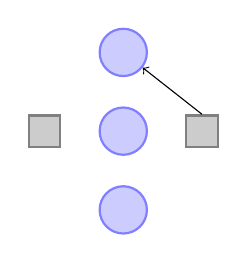
\begin{tikzpicture}
[place/.style={circle,draw=blue!50,fill=blue!20,thick,
inner sep=0pt,minimum size=6mm},
transition/.style={rectangle,draw=black!50,fill=black!20,thick,
inner sep=0pt,minimum size=4mm}]
\node at ( 0,2) [place] (waiting){};
\node at ( 0,1) [place] {};
\node at ( 0,0) [place] {};
\node at ( 1,1) [transition] (1){};
\node at (-1,1) [transition] {};
\draw [->] (1.north) -- (waiting);
\end{tikzpicture}
\end{center}

\subsection*{Klient}
\setlength{\unitlength}{4144sp}%
%
\begingroup\makeatletter\ifx\SetFigFont\undefined%
\gdef\SetFigFont#1#2#3#4#5{%
  \reset@font\fontsize{#1}{#2pt}%
  \fontfamily{#3}\fontseries{#4}\fontshape{#5}%
  \selectfont}%
\fi\endgroup%
\begin{picture}(1207,1568)(1830,-2083)
\put(1845,-689){\makebox(0,0)[lb]{\smash{{\SetFigFont{12}{14.4}{\rmdefault}{\mddefault}{\updefault}{\color[rgb]{0,0,0}+-----+}}}}}

\end{picture}%
\subsection*{Server}
obrazek distribuovana architektura

+--------+\\
| Jabber |\\
| client |     +--------+\\
+--------+     |        |\\
    |          | Jabber |      +..................+\\
    +----------| server |      :                  :\\
               |        |      :                  :\\
               +--------+      :                  :\\
                   |           :     Internet     :\\
                   +-----------:                  :-----------+\\
                               :                  :           |\\
                               :                  :       +--------+\\
                               :                  :       |        |\\
                               :                  :       | Jabber |\\
                               +..................:       | server |--------+\\
                                                          |        |        |\\
                                                          +--------+    +--------+\\
                                                                        | Jabber |\\
                                                                        | client |\\
                                                                        +--------+ \\
\section{Knihovny}
Jabber je realizov�n jako otev?en� XML standart pro instant messaging form�t, proto existuje mnoho programovac�ch jazyk?, kter�m je pr�ce s n�m 
usnadn?na pomoc� knihovny. Mezi nejzn�m?j?� pat?� C (iksemel, libstrophe, Loudmoutn), C++ (gloox, Iris), JAVA (JabberBeans, Smack, JSO, Feridian, Emite, minijingle), 
.NET (Jabber-Net, agsXMPP SDK), Python (JabberPy, PyXMPP, SleekXMPP, Twisted Words), Ruby (XMPP4R, Jabber4R, Jabber::Simple, Jabber::Bot), 
Perl (Net-Jabber) n?kter� n�?e budou lehce rozebr�ny a vyzdvi?eny jejich hlavn� p?ednosti.
\subsection*{iksemel}
\subsection*{JabberBeans}
\subsection*{Jabber-Net}


\subsection*{JabberPy}


\chapter{Dataming}
% \begin{tikzpicture}
% \pgftransformxscale{1.000000}
% \pgftransformyscale{-1.000000}
% \definecolor{dialinecolor}{rgb}{0.000000, 0.000000, 0.000000}
% \pgfsetstrokecolor{dialinecolor}
% \definecolor{dialinecolor}{rgb}{1.000000, 1.000000, 1.000000}
% \pgfsetfillcolor{dialinecolor}
% \pgfsetlinewidth{0.100000\du}
% \pgfsetdash{}{0pt}
% \definecolor{dialinecolor}{rgb}{1.000000, 1.000000, 1.000000}
% \pgfsetfillcolor{dialinecolor}
% \fill (0.568850\du,-138.031250\du)--(0.568850\du,-136.631250\du)--(8.383850\du,-136.631250\du)--(8.383850\du,-138.031250\du)--cycle;
% \definecolor{dialinecolor}{rgb}{0.000000, 0.000000, 0.000000}
% \pgfsetstrokecolor{dialinecolor}
% \draw (0.568850\du,-138.031250\du)--(0.568850\du,-136.631250\du)--(8.383850\du,-136.631250\du)--(8.383850\du,-138.031250\du)--cycle;
% % setfont left to latex
% \definecolor{dialinecolor}{rgb}{0.000000, 0.000000, 0.000000}
% \pgfsetstrokecolor{dialinecolor}
% \node at (4.476350\du,-137.081250\du){debug};
% \definecolor{dialinecolor}{rgb}{1.000000, 1.000000, 1.000000}
% \pgfsetfillcolor{dialinecolor}
% \fill (0.568850\du,-136.631250\du)--(0.568850\du,-132.431250\du)--(8.383850\du,-132.431250\du)--(8.383850\du,-136.631250\du)--cycle;
% \definecolor{dialinecolor}{rgb}{0.000000, 0.000000, 0.000000}
% \pgfsetstrokecolor{dialinecolor}
% \draw (0.568850\du,-136.631250\du)--(0.568850\du,-132.431250\du)--(8.383850\du,-132.431250\du)--(8.383850\du,-136.631250\du)--cycle;
% % setfont left to latex
% \definecolor{dialinecolor}{rgb}{0.000000, 0.000000, 0.000000}
% \pgfsetstrokecolor{dialinecolor}
% \node[anchor=west] at (0.718850\du,-135.931250\du){+id: serial};
% % setfont left to latex
% \definecolor{dialinecolor}{rgb}{0.000000, 0.000000, 0.000000}
% \pgfsetstrokecolor{dialinecolor}
% \node[anchor=west] at (0.718850\du,-135.131250\du){+area: integer};
% % setfont left to latex
% \definecolor{dialinecolor}{rgb}{0.000000, 0.000000, 0.000000}
% \pgfsetstrokecolor{dialinecolor}
% \node[anchor=west] at (0.718850\du,-134.331250\du){+dateadd: timestamp};
% % setfont left to latex
% \definecolor{dialinecolor}{rgb}{0.000000, 0.000000, 0.000000}
% \pgfsetstrokecolor{dialinecolor}
% \node[anchor=west] at (0.718850\du,-133.531250\du){+level: integer};
% % setfont left to latex
% \definecolor{dialinecolor}{rgb}{0.000000, 0.000000, 0.000000}
% \pgfsetstrokecolor{dialinecolor}
% \node[anchor=west] at (0.718850\du,-132.731250\du){+message: text};
% \pgfsetlinewidth{0.100000\du}
% \pgfsetdash{}{0pt}
% \definecolor{dialinecolor}{rgb}{1.000000, 1.000000, 1.000000}
% \pgfsetfillcolor{dialinecolor}
% \fill (10.568850\du,-138.006250\du)--(10.568850\du,-136.606250\du)--(18.768850\du,-136.606250\du)--(18.768850\du,-138.006250\du)--cycle;
% \definecolor{dialinecolor}{rgb}{0.000000, 0.000000, 0.000000}
% \pgfsetstrokecolor{dialinecolor}
% \draw (10.568850\du,-138.006250\du)--(10.568850\du,-136.606250\du)--(18.768850\du,-136.606250\du)--(18.768850\du,-138.006250\du)--cycle;
% % setfont left to latex
% \definecolor{dialinecolor}{rgb}{0.000000, 0.000000, 0.000000}
% \pgfsetstrokecolor{dialinecolor}
% \node at (14.668850\du,-137.056250\du){level};
% \definecolor{dialinecolor}{rgb}{1.000000, 1.000000, 1.000000}
% \pgfsetfillcolor{dialinecolor}
% \fill (10.568850\du,-136.606250\du)--(10.568850\du,-133.206250\du)--(18.768850\du,-133.206250\du)--(18.768850\du,-136.606250\du)--cycle;
% \definecolor{dialinecolor}{rgb}{0.000000, 0.000000, 0.000000}
% \pgfsetstrokecolor{dialinecolor}
% \draw (10.568850\du,-136.606250\du)--(10.568850\du,-133.206250\du)--(18.768850\du,-133.206250\du)--(18.768850\du,-136.606250\du)--cycle;
% % setfont left to latex
% \definecolor{dialinecolor}{rgb}{0.000000, 0.000000, 0.000000}
% \pgfsetstrokecolor{dialinecolor}
% \node[anchor=west] at (10.718850\du,-135.906250\du){+num: integer};
% % setfont left to latex
% \definecolor{dialinecolor}{rgb}{0.000000, 0.000000, 0.000000}
% \pgfsetstrokecolor{dialinecolor}
% \node[anchor=west] at (10.718850\du,-135.106250\du){+name: text};
% % setfont left to latex
% \definecolor{dialinecolor}{rgb}{0.000000, 0.000000, 0.000000}
% \pgfsetstrokecolor{dialinecolor}
% \node[anchor=west] at (10.718850\du,-134.306250\du){+description: text};
% % setfont left to latex
% \definecolor{dialinecolor}{rgb}{0.000000, 0.000000, 0.000000}
% \pgfsetstrokecolor{dialinecolor}
% \node[anchor=west] at (10.718850\du,-133.506250\du){+descriptioncz: text};
% \pgfsetlinewidth{0.100000\du}
% \pgfsetdash{}{0pt}
% \definecolor{dialinecolor}{rgb}{1.000000, 1.000000, 1.000000}
% \pgfsetfillcolor{dialinecolor}
% \fill (0.218950\du,-119.668750\du)--(0.218950\du,-118.268750\du)--(8.418950\du,-118.268750\du)--(8.418950\du,-119.668750\du)--cycle;
% \definecolor{dialinecolor}{rgb}{0.000000, 0.000000, 0.000000}
% \pgfsetstrokecolor{dialinecolor}
% \draw (0.218950\du,-119.668750\du)--(0.218950\du,-118.268750\du)--(8.418950\du,-118.268750\du)--(8.418950\du,-119.668750\du)--cycle;
% % setfont left to latex
% \definecolor{dialinecolor}{rgb}{0.000000, 0.000000, 0.000000}
% \pgfsetstrokecolor{dialinecolor}
% \node at (4.318950\du,-118.718750\du){logarea};
% \definecolor{dialinecolor}{rgb}{1.000000, 1.000000, 1.000000}
% \pgfsetfillcolor{dialinecolor}
% \fill (0.218950\du,-118.268750\du)--(0.218950\du,-114.868750\du)--(8.418950\du,-114.868750\du)--(8.418950\du,-118.268750\du)--cycle;
% \definecolor{dialinecolor}{rgb}{0.000000, 0.000000, 0.000000}
% \pgfsetstrokecolor{dialinecolor}
% \draw (0.218950\du,-118.268750\du)--(0.218950\du,-114.868750\du)--(8.418950\du,-114.868750\du)--(8.418950\du,-118.268750\du)--cycle;
% % setfont left to latex
% \definecolor{dialinecolor}{rgb}{0.000000, 0.000000, 0.000000}
% \pgfsetstrokecolor{dialinecolor}
% \node[anchor=west] at (0.368950\du,-117.568750\du){+num: serial};
% % setfont left to latex
% \definecolor{dialinecolor}{rgb}{0.000000, 0.000000, 0.000000}
% \pgfsetstrokecolor{dialinecolor}
% \node[anchor=west] at (0.368950\du,-116.768750\du){+name: text};
% % setfont left to latex
% \definecolor{dialinecolor}{rgb}{0.000000, 0.000000, 0.000000}
% \pgfsetstrokecolor{dialinecolor}
% \node[anchor=west] at (0.368950\du,-115.968750\du){+description: text};
% % setfont left to latex
% \definecolor{dialinecolor}{rgb}{0.000000, 0.000000, 0.000000}
% \pgfsetstrokecolor{dialinecolor}
% \node[anchor=west] at (0.368950\du,-115.168750\du){+descriptioncz: text};
% \pgfsetlinewidth{0.100000\du}
% \pgfsetdash{}{0pt}
% \definecolor{dialinecolor}{rgb}{1.000000, 1.000000, 1.000000}
% \pgfsetfillcolor{dialinecolor}
% \fill (1.068950\du,-130.018750\du)--(1.068950\du,-128.618750\du)--(7.728950\du,-128.618750\du)--(7.728950\du,-130.018750\du)--cycle;
% \definecolor{dialinecolor}{rgb}{0.000000, 0.000000, 0.000000}
% \pgfsetstrokecolor{dialinecolor}
% \draw (1.068950\du,-130.018750\du)--(1.068950\du,-128.618750\du)--(7.728950\du,-128.618750\du)--(7.728950\du,-130.018750\du)--cycle;
% % setfont left to latex
% \definecolor{dialinecolor}{rgb}{0.000000, 0.000000, 0.000000}
% \pgfsetstrokecolor{dialinecolor}
% \node at (4.398950\du,-129.068750\du){message};
% \definecolor{dialinecolor}{rgb}{1.000000, 1.000000, 1.000000}
% \pgfsetfillcolor{dialinecolor}
% \fill (1.068950\du,-128.618750\du)--(1.068950\du,-122.018750\du)--(7.728950\du,-122.018750\du)--(7.728950\du,-128.618750\du)--cycle;
% \definecolor{dialinecolor}{rgb}{0.000000, 0.000000, 0.000000}
% \pgfsetstrokecolor{dialinecolor}
% \draw (1.068950\du,-128.618750\du)--(1.068950\du,-122.018750\du)--(7.728950\du,-122.018750\du)--(7.728950\du,-128.618750\du)--cycle;
% % setfont left to latex
% \definecolor{dialinecolor}{rgb}{0.000000, 0.000000, 0.000000}
% \pgfsetstrokecolor{dialinecolor}
% \node[anchor=west] at (1.218950\du,-127.918750\du){+id: serial};
% % setfont left to latex
% \definecolor{dialinecolor}{rgb}{0.000000, 0.000000, 0.000000}
% \pgfsetstrokecolor{dialinecolor}
% \node[anchor=west] at (1.218950\du,-127.118750\du){+date: timestamp};
% % setfont left to latex
% \definecolor{dialinecolor}{rgb}{0.000000, 0.000000, 0.000000}
% \pgfsetstrokecolor{dialinecolor}
% \node[anchor=west] at (1.218950\du,-126.318750\du){+fromj: text};
% % setfont left to latex
% \definecolor{dialinecolor}{rgb}{0.000000, 0.000000, 0.000000}
% \pgfsetstrokecolor{dialinecolor}
% \node[anchor=west] at (1.218950\du,-125.518750\du){+toj: text};
% % setfont left to latex
% \definecolor{dialinecolor}{rgb}{0.000000, 0.000000, 0.000000}
% \pgfsetstrokecolor{dialinecolor}
% \node[anchor=west] at (1.218950\du,-124.718750\du){+message: text};
% % setfont left to latex
% \definecolor{dialinecolor}{rgb}{0.000000, 0.000000, 0.000000}
% \pgfsetstrokecolor{dialinecolor}
% \node[anchor=west] at (1.218950\du,-123.918750\du){+subject: text};
% % setfont left to latex
% \definecolor{dialinecolor}{rgb}{0.000000, 0.000000, 0.000000}
% \pgfsetstrokecolor{dialinecolor}
% \node[anchor=west] at (1.218950\du,-123.118750\du){+thread: text};
% % setfont left to latex
% \definecolor{dialinecolor}{rgb}{0.000000, 0.000000, 0.000000}
% \pgfsetstrokecolor{dialinecolor}
% \node[anchor=west] at (1.218950\du,-122.318750\du){+subtype: text};
% \pgfsetlinewidth{0.100000\du}
% \pgfsetdash{}{0pt}
% \definecolor{dialinecolor}{rgb}{1.000000, 1.000000, 1.000000}
% \pgfsetfillcolor{dialinecolor}
% \fill (11.018950\du,-130.918750\du)--(11.018950\du,-129.518750\du)--(18.448950\du,-129.518750\du)--(18.448950\du,-130.918750\du)--cycle;
% \definecolor{dialinecolor}{rgb}{0.000000, 0.000000, 0.000000}
% \pgfsetstrokecolor{dialinecolor}
% \draw (11.018950\du,-130.918750\du)--(11.018950\du,-129.518750\du)--(18.448950\du,-129.518750\du)--(18.448950\du,-130.918750\du)--cycle;
% % setfont left to latex
% \definecolor{dialinecolor}{rgb}{0.000000, 0.000000, 0.000000}
% \pgfsetstrokecolor{dialinecolor}
% \node at (14.733950\du,-129.968750\du){presence};
% \definecolor{dialinecolor}{rgb}{1.000000, 1.000000, 1.000000}
% \pgfsetfillcolor{dialinecolor}
% \fill (11.018950\du,-129.518750\du)--(11.018950\du,-121.318750\du)--(18.448950\du,-121.318750\du)--(18.448950\du,-129.518750\du)--cycle;
% \definecolor{dialinecolor}{rgb}{0.000000, 0.000000, 0.000000}
% \pgfsetstrokecolor{dialinecolor}
% \draw (11.018950\du,-129.518750\du)--(11.018950\du,-121.318750\du)--(18.448950\du,-121.318750\du)--(18.448950\du,-129.518750\du)--cycle;
% % setfont left to latex
% \definecolor{dialinecolor}{rgb}{0.000000, 0.000000, 0.000000}
% \pgfsetstrokecolor{dialinecolor}
% \node[anchor=west] at (11.168950\du,-128.818750\du){+id: serial};
% % setfont left to latex
% \definecolor{dialinecolor}{rgb}{0.000000, 0.000000, 0.000000}
% \pgfsetstrokecolor{dialinecolor}
% \node[anchor=west] at (11.168950\du,-128.018750\du){+date: timestamp};
% % setfont left to latex
% \definecolor{dialinecolor}{rgb}{0.000000, 0.000000, 0.000000}
% \pgfsetstrokecolor{dialinecolor}
% \node[anchor=west] at (11.168950\du,-127.218750\du){+fromj: text};
% % setfont left to latex
% \definecolor{dialinecolor}{rgb}{0.000000, 0.000000, 0.000000}
% \pgfsetstrokecolor{dialinecolor}
% \node[anchor=west] at (11.168950\du,-126.418750\du){+to: text};
% % setfont left to latex
% \definecolor{dialinecolor}{rgb}{0.000000, 0.000000, 0.000000}
% \pgfsetstrokecolor{dialinecolor}
% \node[anchor=west] at (11.168950\du,-125.618750\du){+message: text};
% % setfont left to latex
% \definecolor{dialinecolor}{rgb}{0.000000, 0.000000, 0.000000}
% \pgfsetstrokecolor{dialinecolor}
% \node[anchor=west] at (11.168950\du,-124.818750\du){+name: text};
% % setfont left to latex
% \definecolor{dialinecolor}{rgb}{0.000000, 0.000000, 0.000000}
% \pgfsetstrokecolor{dialinecolor}
% \node[anchor=west] at (11.168950\du,-124.018750\du){+resource: text};
% % setfont left to latex
% \definecolor{dialinecolor}{rgb}{0.000000, 0.000000, 0.000000}
% \pgfsetstrokecolor{dialinecolor}
% \node[anchor=west] at (11.168950\du,-123.218750\du){+presence: text};
% % setfont left to latex
% \definecolor{dialinecolor}{rgb}{0.000000, 0.000000, 0.000000}
% \pgfsetstrokecolor{dialinecolor}
% \node[anchor=west] at (11.168950\du,-122.418750\du){+status: text};
% % setfont left to latex
% \definecolor{dialinecolor}{rgb}{0.000000, 0.000000, 0.000000}
% \pgfsetstrokecolor{dialinecolor}
% \node[anchor=west] at (11.168950\du,-121.618750\du){+priority: integer};
% \pgfsetlinewidth{0.100000\du}
% \pgfsetdash{}{0pt}
% \definecolor{dialinecolor}{rgb}{1.000000, 1.000000, 1.000000}
% \pgfsetfillcolor{dialinecolor}
% \fill (-8.831050\du,-118.118750\du)--(-8.831050\du,-116.718750\du)--(-2.171050\du,-116.718750\du)--(-2.171050\du,-118.118750\du)--cycle;
% \definecolor{dialinecolor}{rgb}{0.000000, 0.000000, 0.000000}
% \pgfsetstrokecolor{dialinecolor}
% \draw (-8.831050\du,-118.118750\du)--(-8.831050\du,-116.718750\du)--(-2.171050\du,-116.718750\du)--(-2.171050\du,-118.118750\du)--cycle;
% % setfont left to latex
% \definecolor{dialinecolor}{rgb}{0.000000, 0.000000, 0.000000}
% \pgfsetstrokecolor{dialinecolor}
% \node at (-5.501050\du,-117.168750\du){userjid};
% \definecolor{dialinecolor}{rgb}{1.000000, 1.000000, 1.000000}
% \pgfsetfillcolor{dialinecolor}
% \fill (-8.831050\du,-116.718750\du)--(-8.831050\du,-114.918750\du)--(-2.171050\du,-114.918750\du)--(-2.171050\du,-116.718750\du)--cycle;
% \definecolor{dialinecolor}{rgb}{0.000000, 0.000000, 0.000000}
% \pgfsetstrokecolor{dialinecolor}
% \draw (-8.831050\du,-116.718750\du)--(-8.831050\du,-114.918750\du)--(-2.171050\du,-114.918750\du)--(-2.171050\du,-116.718750\du)--cycle;
% % setfont left to latex
% \definecolor{dialinecolor}{rgb}{0.000000, 0.000000, 0.000000}
% \pgfsetstrokecolor{dialinecolor}
% \node[anchor=west] at (-8.681050\du,-116.018750\du){+jidbare: text};
% % setfont left to latex
% \definecolor{dialinecolor}{rgb}{0.000000, 0.000000, 0.000000}
% \pgfsetstrokecolor{dialinecolor}
% \node[anchor=west] at (-8.681050\du,-115.218750\du){+date: timestamp};
% \pgfsetlinewidth{0.100000\du}
% \pgfsetdash{}{0pt}
% \definecolor{dialinecolor}{rgb}{1.000000, 1.000000, 1.000000}
% \pgfsetfillcolor{dialinecolor}
% \fill (-9.431050\du,-138.018750\du)--(-9.431050\du,-136.618750\du)--(-1.616050\du,-136.618750\du)--(-1.616050\du,-138.018750\du)--cycle;
% \definecolor{dialinecolor}{rgb}{0.000000, 0.000000, 0.000000}
% \pgfsetstrokecolor{dialinecolor}
% \draw (-9.431050\du,-138.018750\du)--(-9.431050\du,-136.618750\du)--(-1.616050\du,-136.618750\du)--(-1.616050\du,-138.018750\du)--cycle;
% % setfont left to latex
% \definecolor{dialinecolor}{rgb}{0.000000, 0.000000, 0.000000}
% \pgfsetstrokecolor{dialinecolor}
% \node at (-5.523550\du,-137.068750\du){vcard};
% \definecolor{dialinecolor}{rgb}{1.000000, 1.000000, 1.000000}
% \pgfsetfillcolor{dialinecolor}
% \fill (-9.431050\du,-136.618750\du)--(-9.431050\du,-119.618750\du)--(-1.616050\du,-119.618750\du)--(-1.616050\du,-136.618750\du)--cycle;
% \definecolor{dialinecolor}{rgb}{0.000000, 0.000000, 0.000000}
% \pgfsetstrokecolor{dialinecolor}
% \draw (-9.431050\du,-136.618750\du)--(-9.431050\du,-119.618750\du)--(-1.616050\du,-119.618750\du)--(-1.616050\du,-136.618750\du)--cycle;
% % setfont left to latex
% \definecolor{dialinecolor}{rgb}{0.000000, 0.000000, 0.000000}
% \pgfsetstrokecolor{dialinecolor}
% \node[anchor=west] at (-9.281050\du,-135.918750\du){+id: serial};
% % setfont left to latex
% \definecolor{dialinecolor}{rgb}{0.000000, 0.000000, 0.000000}
% \pgfsetstrokecolor{dialinecolor}
% \node[anchor=west] at (-9.281050\du,-135.118750\du){+jid: text};
% % setfont left to latex
% \definecolor{dialinecolor}{rgb}{0.000000, 0.000000, 0.000000}
% \pgfsetstrokecolor{dialinecolor}
% \node[anchor=west] at (-9.281050\du,-134.318750\du){+dateadd: timestamp};
% % setfont left to latex
% \definecolor{dialinecolor}{rgb}{0.000000, 0.000000, 0.000000}
% \pgfsetstrokecolor{dialinecolor}
% \node[anchor=west] at (-9.281050\du,-133.518750\du){+family: text};
% % setfont left to latex
% \definecolor{dialinecolor}{rgb}{0.000000, 0.000000, 0.000000}
% \pgfsetstrokecolor{dialinecolor}
% \node[anchor=west] at (-9.281050\du,-132.718750\du){+given: text};
% % setfont left to latex
% \definecolor{dialinecolor}{rgb}{0.000000, 0.000000, 0.000000}
% \pgfsetstrokecolor{dialinecolor}
% \node[anchor=west] at (-9.281050\du,-131.918750\du){+middle: text};
% % setfont left to latex
% \definecolor{dialinecolor}{rgb}{0.000000, 0.000000, 0.000000}
% \pgfsetstrokecolor{dialinecolor}
% \node[anchor=west] at (-9.281050\du,-131.118750\du){+prefix: text};
% % setfont left to latex
% \definecolor{dialinecolor}{rgb}{0.000000, 0.000000, 0.000000}
% \pgfsetstrokecolor{dialinecolor}
% \node[anchor=west] at (-9.281050\du,-130.318750\du){+suffix: text};
% % setfont left to latex
% \definecolor{dialinecolor}{rgb}{0.000000, 0.000000, 0.000000}
% \pgfsetstrokecolor{dialinecolor}
% \node[anchor=west] at (-9.281050\du,-129.518750\du){+nickname: text};
% % setfont left to latex
% \definecolor{dialinecolor}{rgb}{0.000000, 0.000000, 0.000000}
% \pgfsetstrokecolor{dialinecolor}
% \node[anchor=west] at (-9.281050\du,-128.718750\du){+url: text};
% % setfont left to latex
% \definecolor{dialinecolor}{rgb}{0.000000, 0.000000, 0.000000}
% \pgfsetstrokecolor{dialinecolor}
% \node[anchor=west] at (-9.281050\du,-127.918750\du){+bday: text};
% % setfont left to latex
% \definecolor{dialinecolor}{rgb}{0.000000, 0.000000, 0.000000}
% \pgfsetstrokecolor{dialinecolor}
% \node[anchor=west] at (-9.281050\du,-127.118750\du){+jabberid: text};
% % setfont left to latex
% \definecolor{dialinecolor}{rgb}{0.000000, 0.000000, 0.000000}
% \pgfsetstrokecolor{dialinecolor}
% \node[anchor=west] at (-9.281050\du,-126.318750\du){+title: text};
% % setfont left to latex
% \definecolor{dialinecolor}{rgb}{0.000000, 0.000000, 0.000000}
% \pgfsetstrokecolor{dialinecolor}
% \node[anchor=west] at (-9.281050\du,-125.518750\du){+role: text};
% % setfont left to latex
% \definecolor{dialinecolor}{rgb}{0.000000, 0.000000, 0.000000}
% \pgfsetstrokecolor{dialinecolor}
% \node[anchor=west] at (-9.281050\du,-124.718750\du){+note: text};
% % setfont left to latex
% \definecolor{dialinecolor}{rgb}{0.000000, 0.000000, 0.000000}
% \pgfsetstrokecolor{dialinecolor}
% \node[anchor=west] at (-9.281050\du,-123.918750\du){+mailer: text};
% % setfont left to latex
% \definecolor{dialinecolor}{rgb}{0.000000, 0.000000, 0.000000}
% \pgfsetstrokecolor{dialinecolor}
% \node[anchor=west] at (-9.281050\du,-123.118750\du){+rev: text};
% % setfont left to latex
% \definecolor{dialinecolor}{rgb}{0.000000, 0.000000, 0.000000}
% \pgfsetstrokecolor{dialinecolor}
% \node[anchor=west] at (-9.281050\du,-122.318750\du){+uid: text};
% % setfont left to latex
% \definecolor{dialinecolor}{rgb}{0.000000, 0.000000, 0.000000}
% \pgfsetstrokecolor{dialinecolor}
% \node[anchor=west] at (-9.281050\du,-121.518750\du){+tz: text};
% % setfont left to latex
% \definecolor{dialinecolor}{rgb}{0.000000, 0.000000, 0.000000}
% \pgfsetstrokecolor{dialinecolor}
% \node[anchor=west] at (-9.281050\du,-120.718750\du){+prodid: text};
% % setfont left to latex
% \definecolor{dialinecolor}{rgb}{0.000000, 0.000000, 0.000000}
% \pgfsetstrokecolor{dialinecolor}
% \node[anchor=west] at (-9.281050\du,-119.918750\du){+sotstring: text};
% \pgfsetlinewidth{0.100000\du}
% \pgfsetdash{}{0pt}
% \definecolor{dialinecolor}{rgb}{1.000000, 1.000000, 1.000000}
% \pgfsetfillcolor{dialinecolor}
% \fill (11.093950\du,-119.693750\du)--(11.093950\du,-118.293750\du)--(18.908950\du,-118.293750\du)--(18.908950\du,-119.693750\du)--cycle;
% \definecolor{dialinecolor}{rgb}{0.000000, 0.000000, 0.000000}
% \pgfsetstrokecolor{dialinecolor}
% \draw (11.093950\du,-119.693750\du)--(11.093950\du,-118.293750\du)--(18.908950\du,-118.293750\du)--(18.908950\du,-119.693750\du)--cycle;
% % setfont left to latex
% \definecolor{dialinecolor}{rgb}{0.000000, 0.000000, 0.000000}
% \pgfsetstrokecolor{dialinecolor}
% \node at (15.001450\du,-118.743750\du){xml};
% \definecolor{dialinecolor}{rgb}{1.000000, 1.000000, 1.000000}
% \pgfsetfillcolor{dialinecolor}
% \fill (11.093950\du,-118.293750\du)--(11.093950\du,-114.093750\du)--(18.908950\du,-114.093750\du)--(18.908950\du,-118.293750\du)--cycle;
% \definecolor{dialinecolor}{rgb}{0.000000, 0.000000, 0.000000}
% \pgfsetstrokecolor{dialinecolor}
% \draw (11.093950\du,-118.293750\du)--(11.093950\du,-114.093750\du)--(18.908950\du,-114.093750\du)--(18.908950\du,-118.293750\du)--cycle;
% % setfont left to latex
% \definecolor{dialinecolor}{rgb}{0.000000, 0.000000, 0.000000}
% \pgfsetstrokecolor{dialinecolor}
% \node[anchor=west] at (11.243950\du,-117.593750\du){+id: serial};
% % setfont left to latex
% \definecolor{dialinecolor}{rgb}{0.000000, 0.000000, 0.000000}
% \pgfsetstrokecolor{dialinecolor}
% \node[anchor=west] at (11.243950\du,-116.793750\du){+area: integer};
% % setfont left to latex
% \definecolor{dialinecolor}{rgb}{0.000000, 0.000000, 0.000000}
% \pgfsetstrokecolor{dialinecolor}
% \node[anchor=west] at (11.243950\du,-115.993750\du){+dateadd: timestamp};
% % setfont left to latex
% \definecolor{dialinecolor}{rgb}{0.000000, 0.000000, 0.000000}
% \pgfsetstrokecolor{dialinecolor}
% \node[anchor=west] at (11.243950\du,-115.193750\du){+level: integer};
% % setfont left to latex
% \definecolor{dialinecolor}{rgb}{0.000000, 0.000000, 0.000000}
% \pgfsetstrokecolor{dialinecolor}
% \node[anchor=west] at (11.243950\du,-114.393750\du){+message: text};
% \end{tikzpicture}



\section{Metody dolovani dat}
\section{Dolovani znalosti z databazi}






\chapter{Developer}

\section{Cile}

\section{Slepa ulicka}

\section{knihivna, jazyk}

\section{Jine produkty}


\chapter{Nikdy to nebude naprosto dokonal�}


\chapter{Typografick� a~jazykov� z�sady}

\section{Co to je normovan� str�nka?}

\chapter{Z�v?r}
 % viz. obsah.tex

  % Pouzita literatura
  % ----------------------------------------------
\ifczech
  \bibliographystyle{czechiso}
\else 
  \bibliographystyle{plain}
%  \bibliographystyle{alpha}
\fi
  \begin{flushleft}
  \bibliography{literatura} % viz. literatura.bib
  \end{flushleft}
  \appendix
  
  \chapter{Obsah CD}
\chapter{Manual}
\chapter{Konfigrační soubor}
%\chapter{RelaxNG Schéma konfiguračního soboru}
%\chapter{Plakat}

\chapter{Slovník výrazů}
\begin{description}
\item [DNS] --- Domain Name System
\item [GPG] --- dkshckdsjvlsdjvodsvjdfokj
\item [IM služby] --- dkshckdsjvlsdjvodsvjdfokj
\item [IP] --- Internet Protocol
\item [JEP] --- dkshckdsjvlsdjvodsvjdfokj
\item [JID] --- dkshckdsjvlsdjvodsvjdfokj
\item [SASL] --- dkshckdsjvlsdjvodsvjdfokj
\item [TCP] --- dkshckdsjvlsdjvodsvjdfokj
\item [TLS] --- dkshckdsjvlsdjvodsvjdfokj
\item [WWW] --- dkshckdsjvlsdjvodsvjdfokj
\item [XEP] --- dkshckdsjvlsdjvodsvjdfokj
\item [XML] --- dkshckdsjvlsdjvodsvjdfokj
\item [XMPP] --- dkshckdsjvlsdjvodsvjdfokj
\item [e-mail] --- dkshckdsjvlsdjvodsvjdfokj
\item [jabber] --- dkshckdsjvlsdjvodsvjdfokj
\item [klient] --- dkshckdsjvlsdjvodsvjdfokj
\item [presence] --- dkshckdsjvlsdjvodsvjdfokj
\item [server] --- dkshckdsjvlsdjvodsvjdfokj
\item [stanza] --- dkshckdsjvlsdjvodsvjdfokj
\item [vCard] --- dkshckdsjvlsdjvodsvjdfokj


\end{description}

\chapter{Stanza - základní schéma}


\section{iq}\label{Eiq}

\begin{figure}[h]
\begin{verbatim}
<iq from=""
    to=""
    type="[get,set,result,error]"
    id=""
  Namespace
</ig>
\end{verbatim} 
\caption{Popis elementu \textit{\textless iq/\textgreater}.}
 \label{picIqE}
\end{figure}

\begin{table}[h]
\begin{center}
\begin{tabular}{ l  l  l  l } 
jabber:client & jabber:server& jabber:iq:auth& jabber:iq:register\\ 
jabber:iq:roster& jabber:x:offline& jabber:iq:agent& jabber:iq:agents\\ 
 jabber:x:delay& jabber:iq:version& jabber:iq:time& vcard-temp\\ 
 jabber:iq:private& jabber:iq:search& jabber:iq:oob& jabber:x:oob\\ 
 jabber:iq:admin& jabber:iq:filter& jabber:iq:auth:0k& jabber:iq:browse\\ 
jabber:x:event& jabber:iq:conference& jabber:x:signed& jabber:x:encrypted\\ 
 jabber:iq:gateway& jabber:iq:last& jabber:x:envelope& jabber:x:expire\\ 	
  jabber:xdb:ginsert& jabber:xdb:nslist&\multicolumn{2}{l}{texthttp://www.w3.org/1999/xhtml}
\end{tabular}
\caption{Přehled Namespace elementu \textit{\textless iq/\textgreater}.}
\label{tabNamespaceIqE}
\end{center} 
\end{table}

\newpage
\section{Message}\label{Emessage}

\begin{figure}[h]
\begin{verbatim}
<message from=""
         to=""
         type="[normal,chat,groupchat, headline, error]"
         id=""
  <body>  </body>
  <x xmlns="jabber:x:event">
     <[Offline, Delivered, Displayed, Composing]/>
  <subject>  </subject>
  <thread>   </thread>
  <error>    </error>
  <x>        </x>
</message>
\end{verbatim}  
\caption{Popis elementu \textit{\textless message/\textgreater}.}
 \label{picMessageE}
\end{figure}

\section{Presence}\label{Epresence}
\begin{figure}[h]
\begin{verbatim}
<presence from=""
          to=""
          type="[available, unavailable, probe, subscribe,
                 unsubscribe, subscribed, unsubscribed, error]"
          id=""
  <show>
    [away, chat, dnd, normal, xa]
  </show>
  <status>     </status>
  <priority>   </priority>
  <error>      </error>
</presence>
\end{verbatim} 
\caption{Popis elementu \textit{\textless presence/\textgreater}.}
 \label{picPresenceE}
\end{figure}

\newpage
\section{Přehled průběhu rozšíření}\label{Erozsireni}
\begin{figure}[ht]
\begin{verbatim}
<iq from="uzivatel@jabbim.com" type="set" id="pub1">
   <pubsub xmlns="http://jabber.org/protocol/pubsub">
      <publish node="http://jabber.org/protocol/tune">
         <item>
            <tune xmlns="http://jabber.org/protocol/tune">
               <artist>Daniel Landa</artist>
               <length>255</length>
               <source>Nigredo</source>
               <title>1968</title>
               <track>5</track>
            </tune>
         </item>
      </publish>
   </pubsub>
</iq>
\end{verbatim}  
\caption{Informování server o právě přehrávající písničce.}
 \label{picSPep1}
\end{figure}

\begin{figure}[ht]
\begin{verbatim}
<message from="uzivatel@jabbim.com" type="set"
         to="jabinfo@jabbim.com/bot" id="pub1">
   <event xmlns="http://jabber.org/protocol/pubsub#event">
      <items node="http://jabber.org/protocol/tune">
         <item>
            <tune xmlns="http://jabber.org/protocol/tune">
               <artist>Daniel Landa</artist>
               <length>255</length>
               <source>Nigredo</source>
               <title>1968</title>
               <track>5</track>
            </tune>
         </item>
      </items>
   </event>
</message>
\end{verbatim}  
\caption{Server informuje uživatele podporující rozšíření o stavu \textit{uzivatel@jabbim.com}.}
 \label{picSPep2}
\end{figure}

\begin{figure}[ht]
\begin{verbatim}
<message from="uzivatel@jabbim.com" type="set"
         to="uzivatel@jabbim.com/doma" id="pub2">
   <event xmlns="http://jabber.org/protocol/pubsub#event">
      <items node="http://jabber.org/protocol/tune">
         <item>
            <tune xmlns="http://jabber.org/protocol/tune">
               <artist>Daniel Landa</artist>
               <length>255</length>
               <source>Nigredo</source>
               <title>1968</title>
               <track>5</track>
            </tune>
         </item>
      </items>
   </event>
</message>
\end{verbatim}  
\caption{Server přepošle informace o přehrávané písničce všem otevřeným spojením uživatele \textit{uzivatel@jabbim.com}.}
 \label{picSPep3}
\end{figure}

\begin{figure}[ht]
\begin{verbatim}
<iq from="uzivatel@jabbim.com/prace" type="set" id="pub1">
   <pubsub xmlns="http://jabber.org/protocol/pubsub">
      <publish node="http://jabber.org/protocol/tune">
         <item>
            <tune xmlns="http://jabber.org/protocol/tune"/>
         </item>
      </publish>
   </pubsub>
</iq>
\end{verbatim}  
\caption{Uživatel ukončil \uv{vysílaní} rozšířených zpráv o svém stavu.}
 \label{picSPep4}
\end{figure}

\begin{figure}[ht]
\begin{verbatim}
<message from="uzivatel@jabbim.com"
         to="jabinfo@jabbim.com/bot">
   <event xmlns="http://jabber.org/protocol/pubsub#event">
      <items node="http://jabber.org/protocol/tune">
         <item>
            <tune xmlns="http://jabber.org/protocol/tune"/>
         </item>
      </items>
   </event>
</message>
\end{verbatim}  
\caption{Server informuje klienty o ukončení šíření rozšířeného statusu uživatele \textit{uzivatel@jabbim.com}.}
 \label{picSPep5}
\end{figure}

\chapter{Přehled klientů a jejich rozšíření}\label{Eklient}
...... sdufiysdiufisudfyn df ..

.
zrofj http://xmpp.org/xmpp-software/clients/
..sd.fsdf
\begin{table}[ht]
\subtable{
\centering
\renewcommand{\arraystretch}{1.2}
 {\tiny\tt
\begin{tabular}{ l c c c c c c c c c c} 
\rowcolor[gray]{0.9}
\textbf{Klient}	&\textbf{OS} &\textbf{XEP--60}& \textbf{XEP--163}&\textbf{XEP--80} & \textbf{XEP--92} & \textbf{XEP--107} & \textbf{XEP--108} & \textbf{XEP--118}  & \textbf{XEP--} & \textbf{XEP--}\\
Adium		& 		 & 		    & 		      & 		 & 		     & 			 &		\\
Agile Messenger & 		 & 		    & \\
AQQ		& 		 & 		    & \\ 
Ayttm		& 		 & 		    & 		      & 		 & 		     & 			 &		\\
beejive		& 		 & 		    & 		      & 		 & 		     & 			 &		\\
Beem		& 		 & 		    & 		      & 		 & 		     & 			 &		\\
BitlBee		& 		 & 		    & 		      & 		 & 		     & 			 &		\\
Bombus		& 		 & 		    & 		      & 		 & 		     & 			 &		\\
BuddyMob	& 		 & 		    & 		      & 		 & 		     & 			 &		\\
Chatopus	& 		 & 		    & 		      & 		 & 		     & 			 &		\\
Citron		& 		 & 		    & 		      & 		 & 		     & 			 &		\\
Claros Chat	& 		 & 		    & 		      & 		 & 		     & 			 &		\\
climm		& 		 & 		    & 		      & 		 & 		     & 			 &		\\
Coccinella	& 		 & 		    & 		      & 		 & 		     & 			 &		\\
Crosstalk	& 		 & 		    & 		      & 		 & 		     & 			 &		\\
Digsby		& 		 & 		    & 		      & 		 & 		     & 			 &		\\
eM Client	& 		 & 		    & 		      & 		 & 		     & 			 &		\\
emite		& 		 & 		    & 		      & 		 & 		     & 			 &		\\
Empathy		& 		 & 		    & 		      & 		 & 		     & 			 &		\\
Exodus		& 		 & 		    & 		      & 		 & 		     & 			 &		\\
Finch		& 		 & 		    & 		      & 		 & 		     & 			 &		\\
Gajim 		& 		 & 		    & 		      & 		 & 		     & 			 &		\\
Galaxium	& 		 & 		    & 		      & 		 & 		     & 			 &		\\
glu		& 		 & 		    & 		      & 		 & 		     & 			 &		\\
GNU Freetalk	& 		 & 		    & 		      & 		 & 		     & 			 &		\\
Gossip		& 		 & 		    & 		      & 		 & 		     & 			 &		\\
iChat		& 		 & 		    & 		      & 		 & 		     & 			 &		\\
iJab		& 		 & 		    & 		      & 		 & 		     & 			 &		\\
IM+		& 		 & 		    & 		      & 		 & 		     & 			 &		\\ 
imov Messenger	& 		 & 		    & 		      & 		 & 		     & 			 &		\\
irssi-xmpp	& 		 & 		    & 		      & 		 & 		     & 			 &		\\
Jabbear		& 		 & 		    & 		      & 		 & 		     & 			 &		\\
Jabber Mix Client& 		 & 		    & 		      & 		 & 		     & 			 &		\\
jabber.el	& 		 & 		    & 		      & 		 & 		     & 			 &		\\
Jabbim		& 		 & 		    & 		      & 		 & 		     & 			 &		\\
Jabbim for Android& 		 & 		    & 		      & 		 & 		     & 			 &		\\
Jabiru		& 		 & 		    & 		      & 		 & 		     & 			 &		\\
JAJC		& 		 & 		    & 		      & 		 & 		     & 			 &		\\
Jappix		& 		 & 		    & 		      & 		 & 		     & 			 &		\\ \hline
\end{tabular}} }
\end{table}



\begin{table}[ht]
\subtable{
\centering
\renewcommand{\arraystretch}{1.2}
 {\tiny\tt
\begin{tabular}{ l c c c c c c c c c c} 
\rowcolor[gray]{0.9}
\textbf{Klient}	&\textbf{OS} &\textbf{XEP--60}& \textbf{XEP--163}&\textbf{XEP--80} & \textbf{XEP--92} & \textbf{XEP--107} & \textbf{XEP--108} & \textbf{XEP--118}  & \textbf{XEP--} & \textbf{XEP--}\\

JBuddy Messenger& 		 & 		    & 		      & 		 & 		     & 			 &		\\
Jeti		& 		 & 		    & 		      & 		 & 		     & 			 &		\\
Jitsi (SIP Communicator)& 	 & 		    & 		      & 		 & 		     & 			 &		\\
JWChat		& 		 & 		    & 		      & 		 & 		     & 			 &		\\
Kadu		& 		 & 		    & 		      & 		 & 		     & 			 &		\\
Kopete		& 		 & 		    & 		      &			 & 		     & 			 &		\\
Lampiro		& 		 & 		    & 		      & 		 & 		     & 			 &		\\
m-im		& 		 & 		    & 		      & 		 & 		     & 			 &		\\
mcabber		& 		 & 		    & 		      & 		 & 		     & 			 &		\\
mChat		& 		 & 		    & 		      & 		 & 		     & 			 &		\\
Miranda IM	& 		 & 		    & 		      & 		 & 		     & 			 &		\\
Monal IM	& 		 & 		    & 		      & 		 & 		     & 			 &		\\
OctroTalk	& 		 & 		    & 		      & 		 & 		     & 			 &		\\
OneTeam		& 		 & 		    & 		      & 		 & 		     & 			 &		\\
OneTeam for iPhone& 		 & 		    & 		      & 		 & 		     & 			 &		\\
Oyo		& 		 & 		    & 		      & 		 & 		     & 			 &		\\
Pandion		& 		 & 		    & 		      & 		 & 		     & 			 &		\\
Poezio		& 		 & 		    & 		      & 		 &      	     & 			 &		\\
Pidgin		& 		 & 		    & 		      & 		 & 		     & 			 &		\\
Prodromus	& 		 & 		    & 		      & 		 & 		     & 			 &		\\
Psi		& 		 & 		    & 		      & 		 & 		     & 			 &		\\
Psi+		& 		 & 		    & 		      & 		 & 		     & 			 &		\\
Quiet Internet Pager (QIP)& 	 & 		    & 		      & 		 & 		     & 			 &		\\
qutIM		& 		 & 		    & 		      & 		 & 		     & 			 &		\\
saje		& 		 & 		    & 		      & 		 & 		     & 			 &		\\
SamePlace	& 		 & 		    & 		      & 		 & 		     & 			 &		\\
Sim-IM		& 		 & 		    & 		      & 		 & 		     & 			 &		\\
Slimster	& 		 & 		    & 		      & 		 & 		     & 			 &		\\
SoapBox Communicator& 		 & 		    & 		      & 		 & 		     & 			 &		\\
Spark		& 		 & 		    & 		      & 		 & 		     & 			 &		\\
SparkWeb	& 		 & 		    & 		      & 		 & 		     & 			 &		\\
Synapse		& 		 & 		    & 		      & 		 & 		     & 			 &		\\
Talkonaut	& 		 & 		    & 		      & 		 & 		     & 			 &		\\
Tigase Messenger& 		 & 		    & 		      & 		 & 		     & 			 &		\\
Tigase Minichat	& 		 & 		    & 		      & 		 & 		     & 			 &		\\
Tkabber		& 		 & 		    & 		      & 		 & 		     & 			 &		\\
Tlen		& 		 & 		    & 		      & 		 & 		     & 			 &		\\ 
Trillian	& 		 & 		    & 		      & 		 & 		     & 			 &		\\
TrophyIM	& 		 & 		    & 		      & 		 & 		     & 			 &		\\
V\&V Messenger	& 		 & 		    & 		      & 		 & 		     & 			 &		\\
Vacuum-IM	& 		 & 		    & 		      & 		 & 		     & 			 &		\\
Vayusphere	& 		 & 		    & 		      & 		 & 		     & 			 &		\\
WTW		& 		 & 		    & 		      & 		 & 		     & 			 &		\\
Xabber		& 		 & 		    & 		      & 		 & 		     & 			 &		\\
xmppchat	& 		 & 		    & 		      & 		 & 		     & 			 &		\\
Yambi		& 		 & 		    & 		      & 		 & 		     & 			 &		\\
Yaxim		& 		 & 		    & 		      & 		 & 		     & 			 &		\\ \hline
\end{tabular}} }
\caption{Přehled podporovaných rozšíření u jednotlivých klientů.}
\label{tabEklient}

\end{table} % viz. prilohy.tex
\end{document}
